\documentclass[a4paper, titlepage]{article}
\usepackage[left=2cm,right=2cm,
    top=2cm,bottom=2cm,bindingoffset=0cm]{geometry}
    
\usepackage{pscyr}
\DeclareSymbolFont{T2Aletters}{\encodingdefault}{\rmdefault}{m}{it}
\usepackage[warn]{mathtext}          % русские буквы в формулах, с предупреждением
\usepackage[T2A]{fontenc}            % внутренняя кодировка  TeX
\usepackage[utf8x]{inputenc}         % кодовая страница документа
\usepackage[english, russian]{babel} % локализация и переносы
\usepackage{indentfirst}   % русский стиль: отступ первого абзаца раздела
\usepackage{misccorr}      % точка в номерах заголовков
\usepackage{cmap}          % русский поиск в pdf
\usepackage{color}
\usepackage{graphicx}      % Работа с графикой \includegraphics{}
\usepackage{psfrag}        % Замена тагов на eps картинкаx
\usepackage{caption2}      % Работа с подписями для фигур, таблиц и пр.
\usepackage{color, soul}   % Разряженный текст \so{} и подчеркивание \ul{}
\usepackage{soulutf8}      % Поддержка UTF8 в soul
\usepackage{fancyhdr}      % Для работы с колонтитулами
\usepackage{multirow}      % Аналог multicolumn для строк
\usepackage{ltxtable}      % Микс tabularx и longtable
\usepackage{paralist}      % Списки с отступом только в первой строчке
\usepackage{longtable}
\usepackage{tabularx}
\usepackage{listings}      % листинги
\usepackage[perpage]{footmisc} % Нумерация сносок на каждой странице с 1

\usepackage{hyperref}
\hypersetup{colorlinks,urlcolor=blue}

\usepackage{amsmath}
\usepackage{amsfonts}
\usepackage{amssymb}

\usepackage{float}
\graphicspath{{images/}}
\usepackage{multirow}
\usepackage{hyperref}
\usepackage{cite}
\usepackage{verbatim} % блоки комментариев \begin{comment}
\usepackage{icomma}  % В России для разделения целой части цисла от дробной используется запятая '','', в англоязычных странах используется точка ''.''. Если следовать русской традиции набора чисел, используя в качестве разделителя запятую, то получается большой пробел меджу запятой и дробной частью, т.к. LaTeX добавляет небольшой пробел после запятой. Пакет icomma позволяет убрать этот эффект

\usepackage{listings}

\newcommand*\dd{\mathop{}\!\mathrm{d}}
\newcommand*\Dd[1]{\mathop{}\!\mathrm{d^#1}}
\newcommand*\Cyr[1]{\text{\textit{#1}}}


\definecolor{dkgreen}{rgb}{0,0.6,0}
\definecolor{gray}{rgb}{0.5,0.5,0.5}
\definecolor{mauve}{rgb}{0.58,0,0.82}

\title{Отчет}
\author{Крамарев А.Г.}
\renewcommand{\lstlistingname}{Листинг}
\newcommand{\Code}{\fontsize{12}{15}\selectfont}

\lstset{ 
  language=Java,                % Язык программирования 
  %numbers=left,
  numberstyle=\color{gray},
  frame=single,
  title=\lstname,
  rulecolor=\color{black},  
  keywordstyle=\color{blue},          % Стиль ключевых слов
  commentstyle=\color{dkgreen},       % Стиль комментариев
  stringstyle=\color{mauve},
  extendedchars=\true,
  inputencoding=utf8,
  basicstyle=\Code\ttfamily,
  showtabs=\true,
  showspaces=\true,
  columns=fixed,
  breaklines=true,                        % Automatic line breaking?
  breakatwhitespace=true,                % Automatic breaks only at whitespace?
  keepspaces=true,
  extendedchars=\true,
  inputencoding=utf8x,
  literate={а}{{\selectfont\char224}}1
{б}{{\selectfont\char225}}1
{в}{{\selectfont\char226}}1
{г}{{\selectfont\char227}}1
{д}{{\selectfont\char228}}1
{е}{{\selectfont\char229}}1
{ё}{{\"e}}1
{ж}{{\selectfont\char230}}1
{з}{{\selectfont\char231}}1
{и}{{\selectfont\char232}}1
{й}{{\selectfont\char233}}1
{к}{{\selectfont\char234}}1
{л}{{\selectfont\char235}}1
{м}{{\selectfont\char236}}1
{н}{{\selectfont\char237}}1
{о}{{\selectfont\char238}}1
{п}{{\selectfont\char239}}1
{р}{{\selectfont\char240}}1
{с}{{\selectfont\char241}}1
{т}{{\selectfont\char242}}1
{у}{{\selectfont\char243}}1
{ф}{{\selectfont\char244}}1
{х}{{\selectfont\char245}}1
{ц}{{\selectfont\char246}}1
{ч}{{\selectfont\char247}}1
{ш}{{\selectfont\char248}}1
{щ}{{\selectfont\char249}}1
{ъ}{{\selectfont\char250}}1
{ы}{{\selectfont\char251}}1
{ь}{{\selectfont\char252}}1
{э}{{\selectfont\char253}}1
{ю}{{\selectfont\char254}}1
{я}{{\selectfont\char255}}1
{А}{{\selectfont\char192}}1
{Б}{{\selectfont\char193}}1
{В}{{\selectfont\char194}}1
{Г}{{\selectfont\char195}}1
{Д}{{\selectfont\char196}}1
{Е}{{\selectfont\char197}}1
{Ё}{{\"E}}1
{Ж}{{\selectfont\char198}}1
{З}{{\selectfont\char199}}1
{И}{{\selectfont\char200}}1
{Й}{{\selectfont\char201}}1
{К}{{\selectfont\char202}}1
{Л}{{\selectfont\char203}}1
{М}{{\selectfont\char204}}1
{Н}{{\selectfont\char205}}1
{О}{{\selectfont\char206}}1
{П}{{\selectfont\char207}}1
{Р}{{\selectfont\char208}}1
{С}{{\selectfont\char209}}1
{Т}{{\selectfont\char210}}1
{У}{{\selectfont\char211}}1
{Ф}{{\selectfont\char212}}1
{Х}{{\selectfont\char213}}1
{Ц}{{\selectfont\char214}}1
{Ч}{{\selectfont\char215}}1
{Ш}{{\selectfont\char216}}1
{Щ}{{\selectfont\char217}}1
{Ъ}{{\selectfont\char218}}1
{Ы}{{\selectfont\char219}}1
{Ь}{{\selectfont\char220}}1
{Э}{{\selectfont\char221}}1
{Ю}{{\selectfont\char222}}1
{Я}{{\selectfont\char223}}1
}

\begin{document} % Маркер начала документа
\fontsize{14}{16pt}\selectfont

\maketitle % Создать титульный лист на основе данных в заголовке документа

\section{Исходные данные}


\begin{equation*}
\begin{cases}
	F = m a \\
\end{cases}
\Rightarrow
\begin{cases}
	m\ddot{x} + \alpha\dot{x} = 0 \\
	m\ddot{y} + \alpha\dot{y} = - mg
\end{cases}
\end{equation*}

Обозначим $\mu = \dfrac{\alpha}{m}$, получим
\begin{equation}
\label{eq:ish}
\begin{cases}
    \ddot{x} + \mu\dot{x} = 0 \\
    \ddot{y} + \mu\dot{y} = -g \\
\end{cases}
\Rightarrow
\begin{cases}
    \ddot{x} = -\mu\dot{x} \\
    \ddot{y} = -\mu\dot{y} - g
\end{cases}
\end{equation}

Сначала найдем функцию скорости от времени $v_x(t) = \dot{x}$ и $v_y(t)=\dot{y}$. Подставляя в уравнения \ref{eq:ish}, получим:
\begin{equation}
\label{eq:speed-diff}
\begin{cases}
    \dot{x} = v_x \\
    \dot{y} = v_y
\end{cases}
\\
\begin{cases}
    \dot{v_x} = -\mu v_x \\
    \dot{v_y} = -\mu v_y - g
\end{cases}
\\
\begin{cases}
    \dfrac{\dd v_x}{\dd t} = -\mu v_x  \\[1em]
    \dfrac{\dd v_y}{\dd t} = -\mu v_y - g
\end{cases}
\end{equation}

\section{Обезразмеривание}


\subsection{Скорость}
За характерную скорость примем начальную скорость
$$ v_{\Cyr{хар}} = v_0 $$
$$ v = \hat{v} \cdot v_0 $$

\subsection{Время}
В качестве характерного времени примем время полета в условиях отсутствия сопротивления воздуха. Время полета в этом случае равна сумме равных интервалов времени подъема и времени падения снаряда.
Время подъема на максимальную высоту определяется из условия, что вертикальная составляющая мгновенной скорости равна нулю
$$ v_y = v_0 \sin{\alpha}-gt_{h\,max} = 0 $$
из этого уравнения получим время подъема:
$$ t_{h\,max} = \frac{v_0\sin{\alpha}}{g} $$
Имеем расчетное время полета:
$$ t_{\Cyr{хар}} = 2t_{h\,max} = \frac{2 v_0\sin{\alpha}}{g} $$
$$ t = \hat{t} \cdot \frac{2 v_0\sin{\alpha}}{g} $$

Обезразмерим первое уравнение из \ref{eq:speed-diff}:
$$ \dfrac{\dd \hat{v}_x \cdot v_0}{\dd \hat{t} \cdot \dfrac{2 v_0 \sin{\alpha}}{g} } = -\mu \hat{v}_x v_0 $$
аналогично второе:
$$ \dfrac{\dd \hat{v}_y \cdot v_0}{\dd \hat{t} \cdot \dfrac{2 v_0 \sin{\alpha}}{g} } = -\mu \hat{v}_y v_0 - g $$
система уравнений \ref{eq:speed-diff} в безразмерных величинах:
\begin{align*}
\begin{cases}
    \dfrac{\dd \hat{v}_x}{\dd \hat{t}} = -\dfrac{2 \mu v_0\sin{\alpha}}{g}\hat{v}_x &= F_{\hat{v}_x}(t,\hat{v}_x)\\[1em]
    \dfrac{\dd \hat{v}_y}{\dd \hat{t}} = -\dfrac{2 \mu v_0\sin{\alpha}}{g}\hat{v}_y - 2\sin{\alpha} &= F_{\hat{v}_y}(t, \hat{v}_y)
\end{cases}
\end{align*}
при этом начальный величины безразмерных скоростей равны $ \hat{v}_{x0} = (v_0\cos{\alpha}) / v_0 = \cos{\alpha} $, $\hat{v}_{y0} = \sin{\alpha} $.

\subsection{Длина}
Решением уравнений будет функция обезразременных координат от безразмерного времени. Физические величины координат вычисляются как:
$$
    x = \hat{x} \cdot t_\Cyr{хар} \cdot v_\Cyr{хар} = \hat{x} \cdot \frac{2 v_0\sin{\alpha}}{g} \cdot v_0 = \hat{x} \cdot \frac{2 v_0^2\sin{\alpha}}{g}
$$
и аналогично
$$
    y = \hat{y} \cdot \frac{2 v_0^2\sin{\alpha}}{g}
$$


\section{Реализация}
Задача сводится к численному решению дифференциального уравнения
$$ \frac{\dd y}{\dd t} = F(y,t) $$
права часть уравнения будем задавать реализациями интерфейса \lstinline|F|:
\begin{lstlisting}[language=java]
public interface F {
    double eval(double t, double y);
}
\end{lstlisting}

схемы решения реализуют интерфейс \lstinline|Scheme|:
\begin{lstlisting}[language=java]
public interface Scheme {
    /**
     * Вычисляет следущее значение функции y
     * решения дифференциального уравнения
     *         dy/dt = f(y,t)
     * @param f     правая часть уравнения
     * @param t1    время t1
     * @param y1    значение y в момент времени t1
     * @param t2    время в которой вычисляется значение y
     * @return значение y в момент времени t2
     */
    double y2(F f, double t1, double y1, double t2);
}
\end{lstlisting}

В данной задаче для вычисления координат точки в следующий момент времени для каждой отдельной координаты необходимо применить численный метод. Правой частью дифференциального уравнения
\begin{equation}
 \label{eq:diffx}
 \frac{\dd x}{\dd t} = v(t)
\end{equation}

является функция скорости $v(t)$, которая, в свою очередь, также вычисляется численным методом из уравнения
\begin{equation}
 \label{eq:diffv}
 \frac{\dd v}{\dd t} = F(v,t)
\end{equation}


Для решения такой задачи правая часть уравнения \ref{eq:diffx} представляется в виде прокси-объекста \lstinline|Fnum|:
\begin{lstlisting}
public class Fnum implements F {
    ...
    public Fnum(Scheme scheme, F f, double t0, double f0) { ... }
    ...
    @Override
    public double eval(double t, double x) {
        // вычисление значения функции численным методом
        ...
    }
\end{lstlisting}
Используемая схема для решения \ref{eq:diffx} при получении необходимого значения $v(t_{n+1})$ правой части инициирует расчет из уравнения \ref{eq:diffv}, численным методом по схеме, переданной при конструировании \lstinline|Fnum|. Конкретная реализация \lstinline|Fnum| ``помнит'' только последнее вычисленное значение функции, что накладывает следующее ограничение: все реализации схем должны получать значения только в порядке возрастания \lstinline|t|. Однако данный подход позволяет отделить схему расчета от задачи, и позволяет очень гибко добавлять новые схемы. Для этого достаточно добавить новую реализацию интерфейса \lstinline|Scheme|.

\section{Схемы}
Ниже расмотренные некоторые методы на примере решения уравнения $$ \frac{\dd y}{\dd t} = F(y,t) $$

\subsection{Метод Эйлера}
$$ y_{n+1} = y_n + \Delta t F(t_n, y_n) $$
\begin{lstlisting}
public class Euler implements Scheme {
    @Override
    public double y2(F f, double t1, double y1, double t2) {
        return y1 + (t2 - t1) * f.eval(t1, y1);
    }
}
\end{lstlisting}

\subsection{Предиктор-корректор}

\begin{equation*}
\begin{array}{l}
\tilde{y}_{n+1} = y_n + \Delta t F(t_n, y_n) \\[0.5em]
y_{n+1} = y_n + \frac{1}{2}\Delta t (F(t_n, y_n)) + F(t_{n+1}, \tilde{y}_{n+1})) )
\end{array}
\end{equation*}
\begin{lstlisting}
public class PredictorCorrector implements Scheme {
    public double y2(F f, double t1, double y1, double t2) {
        double dt = t2 - t1;
        double f1 = f.eval(t1, y1);
        double y_predictor = y1 + dt * f1;
        return y1 + dt / 2 * (f1 + f.eval(t2, y_predictor));
    }
}
\end{lstlisting}

\subsection{Метод Рунге "--- Кутты}
\begin{equation*}
\begin{array}{l}
y_{n+1} = y_n + \frac{\Delta t}{6}(k_1 + 2k_2 + 2k_3 + k_4) \\[0.4em]
k_1 = F(t_n, y_n) \\[0.4em]
k_2 = F(t_n + \frac{\Delta t}{2}, y_n + \frac{\Delta t}{2}k_1) \\[0.4em]
k_3 = F(t_n + \frac{\Delta t}{2}, y_n + \frac{\Delta t}{2}k_2) \\[0.4em]
k_4 = F(t_n+ \Delta t, y_n + \Delta t k_3)
\end{array}
\end{equation*}
\begin{lstlisting}
public class RungeKutta implements Scheme {
    public double y2(F f, double t1, double y1, double t2) {
        double h2 = t2 - t1, h = h2 / 2;
        double k1 = f.eval(t1, y1),
               k2 = f.eval(t1 + h, y1 + h * k1),
               k3 = f.eval(t1 + h, y1 + h * k2),
               k4 = f.eval(t1 + h2, y1 + h2 * k3);
        return y1 + h2 / 6 * (k1 + 2 * k2 + 2 * k3 + k4);
    }
}
\end{lstlisting}

\section{Аналитическое решение}
Аналитическое решение системы уравнений \ref{eq:ish} найдем используя программный пакет Mathematica:
\begin{lstlisting}[language=mathematica]
DSolve[{
  x''[t] == -\[Mu] x'[t],
  y''[t] == -\[Mu] y'[t] - g,
  x[0] == 0, x'[0] == v0 Cos[\[Alpha]],
  y[0] == 0, y'[0] == v0 Sin[\[Alpha]]
  }, {x[t], y[t]}, t] // Expand
\end{lstlisting}

\begin{equation*}
\begin{array}{l}
x(t)\to \dfrac{\text{v0} \cos (\alpha )}{\mu }-\dfrac{\text{v0} \cos (\alpha ) e^{\mu  (-t)}}{\mu }, \\[0.7em]
y(t)\to \dfrac{g}{\mu ^2}-\dfrac{g e^{\mu  (-t)}}{\mu ^2}-\dfrac{g t}{\mu }-\dfrac{\text{v0} \sin (\alpha ) e^{\mu  (-t)}}{\mu }+\dfrac{\text{v0} \sin (\alpha )}{\mu }
\end{array}
\end{equation*}

\section{Результаты}

\begin{figure}[H]
\caption{Сравнение со схемой Эйлера}
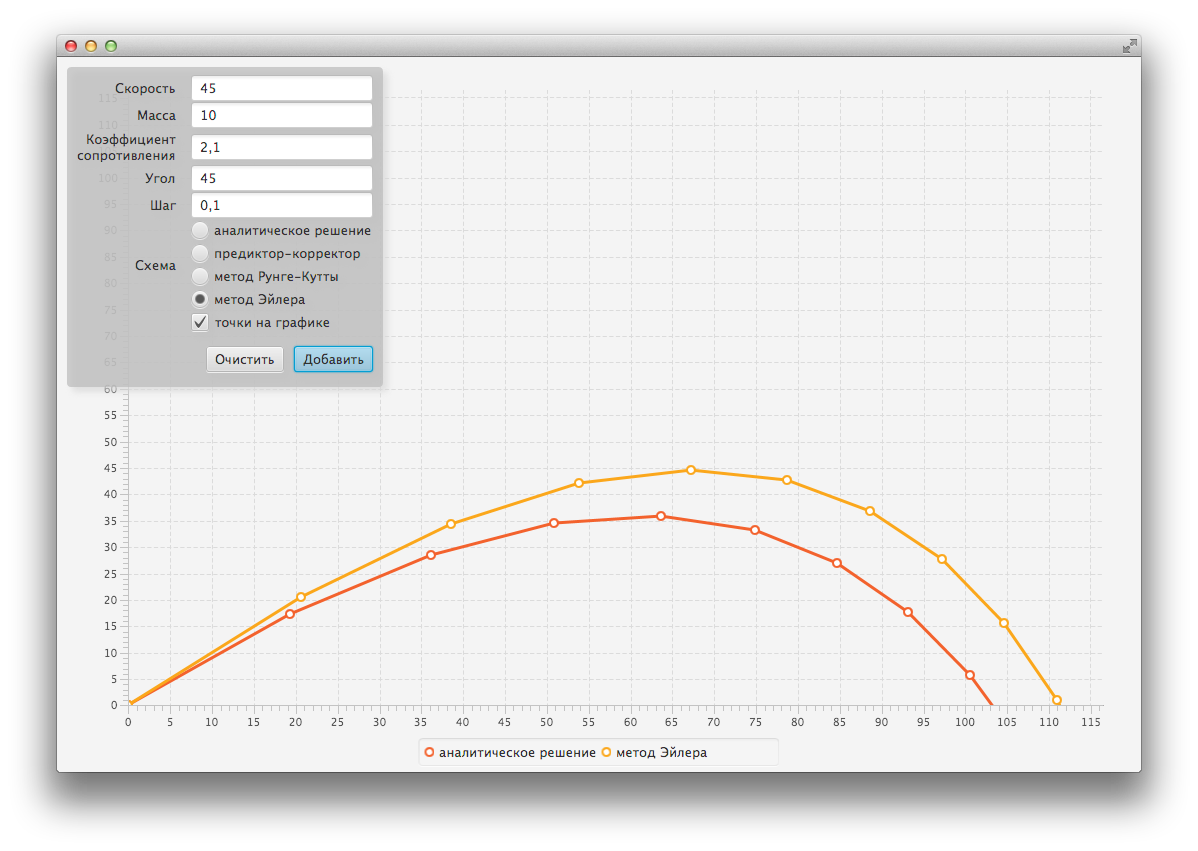
\includegraphics[width=\textwidth]{euler}
\end{figure}

\begin{figure}[H]
\caption{Сравнение со схемой Предиктор-Корректор}
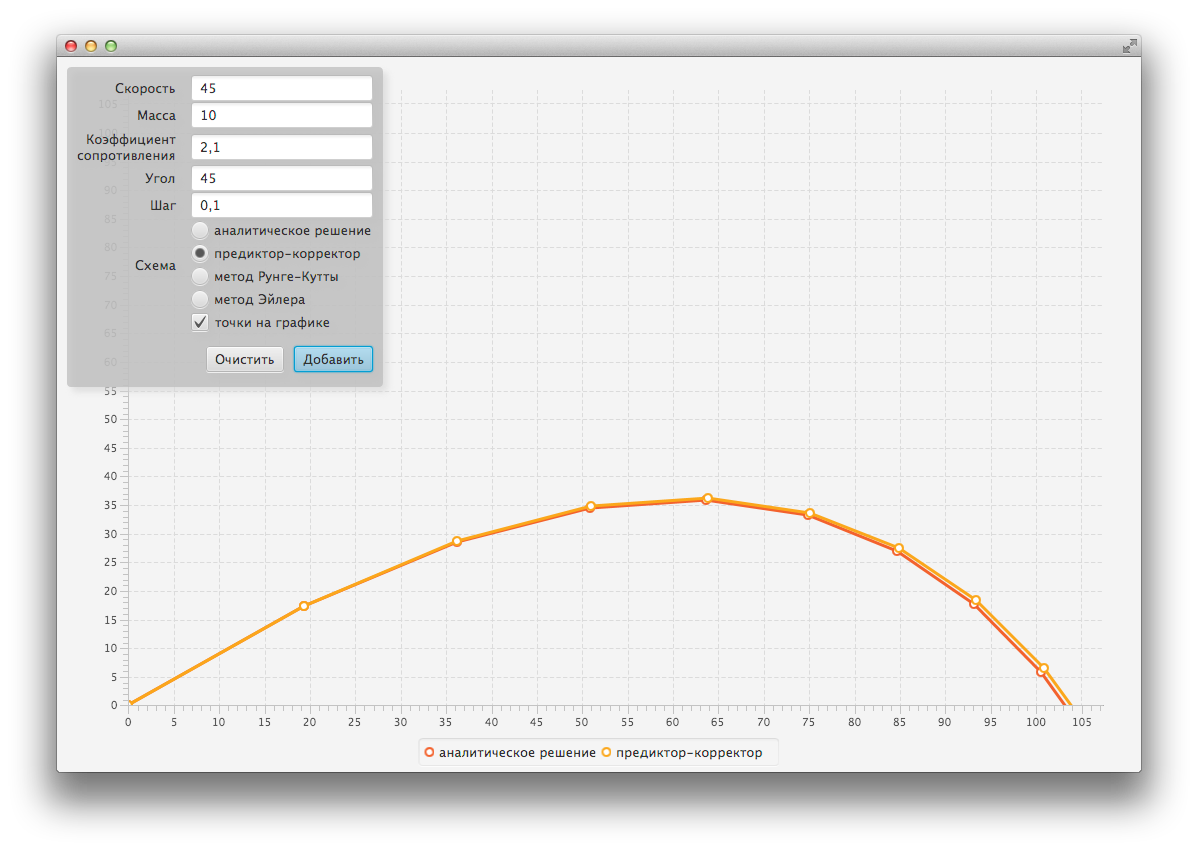
\includegraphics[width=\textwidth]{p-corrector}
\end{figure}


\begin{figure}[H]
\caption{Сравнение с методом Рунге "--- Кутты}
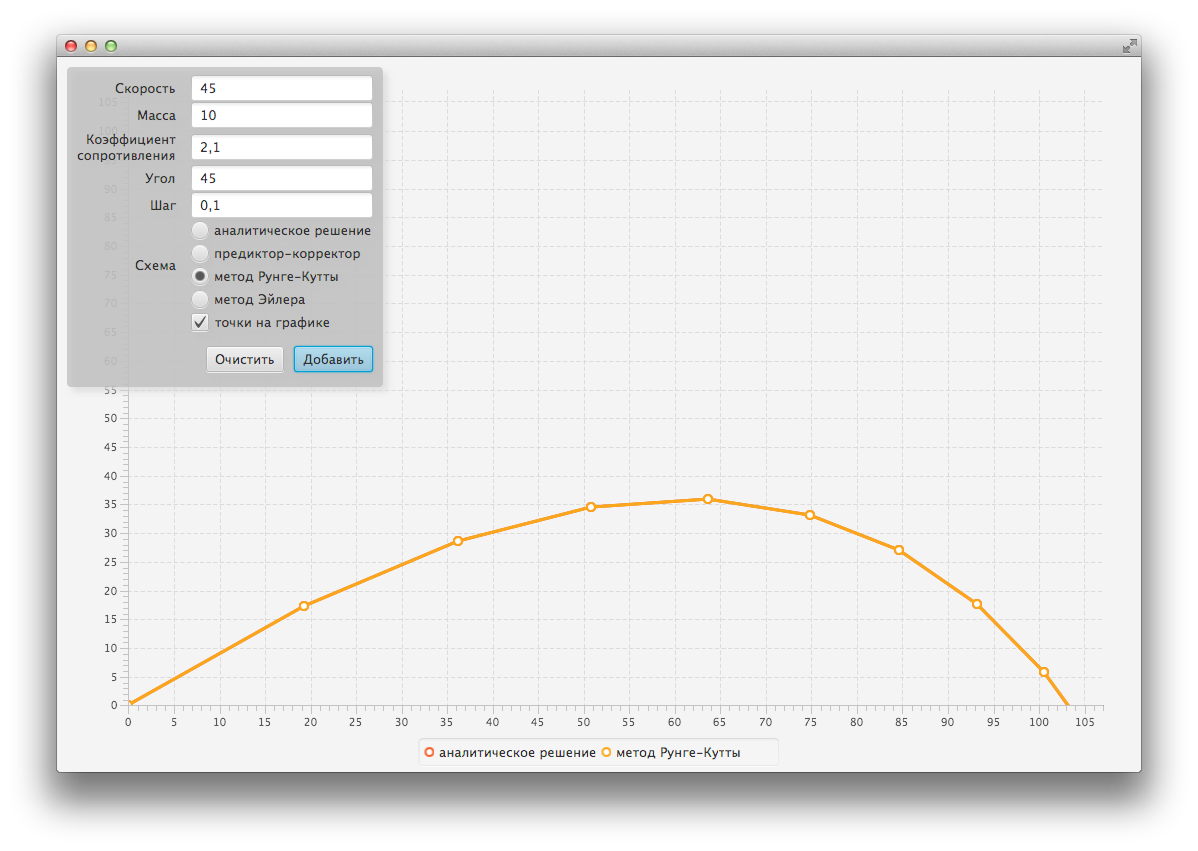
\includegraphics[width=\textwidth]{r-kutta}
\end{figure}


\end{document} % Маркер завершения документа